\documentclass{article}
\usepackage[utf8]{inputenc}
\usepackage{setspace}
\usepackage{amsmath}
\usepackage{graphicx}

\title{Bayesian Analysis of Mass Shooting Fatalities}
\author{Christopher Danko}
\date{April 2020}

\begin{document}


\maketitle
\doublespacing

\section{Abstract}
This paper investigates how states with different gun laws have different rates of mass shooting fatalities. First I use a Bayesian data analysis to demonstrate that there is a significant difference between states with strong gun laws and states with weak gun laws  Using data collected by the Gun Violence Archive for the years 2013-2019 provided to me by an associate, Devin Hughes, I used the information on fatalities to create a statistical experiment to determine whether or not states with strong gun laws have less mass shooting fatalities proportional to their population. A binomial test on each year demonstrates that in five out of eight years, states with strong gun laws have significantly less mass shooting fatalities. This result is consistent with expectations, as gun law advocates would expect states with strong gun laws to have less shooting fatalities per capita than states with weak gun laws. I also use a Monte Carlo Markov Chain model to simulate the posterior distribution of the probability that given a mass shooting fatality has occurred, the fatality occurs in a state with strong gun laws. These findings are consistent with expectations, as advocates of stronger gun laws would expect these laws to result in less lethal mass shootings. Gun laws are expected to reduce the number of high-capacity and high-fire rate firearms in circulation. This effect is expected to result in less total shots fired during a mass shooting, as potential shooters will be forced to resort to less effective firearms. These results contradict expectations of ‘Good Guy With a Gun’ theorists, who argue that reducing access to firearms makes people more vulnerable to mass shooters, who will find ways to obtain lethal firearms regardless of laws. Under these expectations, stronger gun laws should either increase or have no significant effect on fatalities during mass shootings.

\section{Introduction}
The topic of mass murder, and mass shootings specifically, has been mostly ignored–even among criminologists–until fairly recently \cite{1}. Searches of academic databases including JSTOR and Google Scholar did not yield any previous regression analyses of the effect of gun laws on mass shootings in the United States. Most scholarship around mass shootings has instead focused on the effects of public mass shootings on the public debate around gun control laws \cite{2} and the purported links between mental illness and mass shootings \cite{3}.

The definition of mass shooting used here is the definition used by the Gun Violence Archive (GVA), where the data was obtained from. The GVA defines a mass shooting as an incident where 4 or more are injured or killed, not including the shooter. Noteworthy here is equal importance given to counting the number of injured in a shooting in addition to those killed in a mass shooting incident. This means that there are a number of mass shootings that had no fatalities.

A state is classified as having "strong" gun laws or "weak" gun laws based on the Giffords Gun Law Center grades \cite{4}. A state with an A, B, or C rating is considered "strong" and a D or F rating would be considered weak. The cutoff of a C rating is chosen because there is a fairly significant difference between the gun laws in C states and those in D states. Take Florida, a C- rated state as of 2018. Florida has a mandatory waiting period of 3 days, a minimum firearm and ammunition purchasing age of 21, ammunition restrictions \footnote{Florida prohibits the manufacture, sale, delivery, and possession of ammunition types such as armor-piercing bullets, exploding shells, bolo shells, and flechette shells \cite{7}}, and an extreme risk protection order law \footnote{Extreme risk protection order laws allow law enforcement officials to petition courts to obtain civil orders that prevent dangerous persons for accessing firearms to up one year \cite{8}} \cite{5}. North Carolina, a D-rated state, has none of these laws. However, it does have a universal background check requirement for purchasing handguns \cite{6}. This cutoff selection also has the nice property that it creates a fairly even distribution of population between the two groups. A table of states and their Giffords Gun Law Center Ratings is provided in Appendix A. 

The relationship between stronger gun laws and the number of mass shootings is important to identify for policy-makers. If these laws demonstrably reduce the number of mass shootings that take place, that may be a justification for implementing them. If these policies do not reduce the number of mass shootings or other forms of gun violence, they may not be worth implementing. 

This paper chooses to explore the fatality rate of mass shootings for three reasons. Theoretically, stricter gun laws–such as ones that completely ban AR-15s could have no effect on the number of mass shootings and one would conclude that stronger gun laws have no effect on mass shootings. However, mass shooters may be forced to use pistols or other low-capacity, low-fire rate firearms which would lead to fewer fatalities and injuries per shooting. This approach would capture this hypothetical effect, whereas the other approach would not. If stronger gun laws demonstrably reduce the number of casualties per mass shooting, that may be a justification for implementing them.

Second, as the Gun Violence Prevention data set shows, 2642 people have been killed and 9766 people have been injured since 2013. If stronger gun laws reduce the total number of people killed in mass shootings, that is a justification for implementing them.

Finally, there is a clear impact of mass shootings on the public discourse around gun violence. As McGinty, et al. found, being exposed to stories about mass shootings made experiment participants more likely to support stronger firearm restrictions and develop more negative attitudes towards people with mental illnesses \cite{2}. Mass shootings have clear psychological impacts on people that influence their political beliefs and attitudes. If stronger gun laws reduce the severity of events causing psychological stress, that is a justification for implementing them.

\section{Data}
Explain:
How GVPedia Data is collected
What variables the data tracks

\section{Methods}

This paper uses binomial tests to establish statistical difference between the two groups. The null hypothesis for this test is that the distribution of mass shooting fatalities should be equal to the distribution of population \footnote{Population estimates come from the U.S. Census Bureau. U.S. territories are excluded from all population ratio estimates}. If states with strong gun laws contain 50$\%$ of the population, we expect them to contain 50$\%$ of mass shooting fatalities.

The binomial test statistic is calculated by

\begin{equation}
\sum_{i=k}^{N} \binom{N}{i}p^{i}(1-p)^{N-i}
\end{equation}

Where $N$ is the total number of mass shooting fatalities in the particular year, $k$ is the number of mass shooting fatalities that occurred in states with strong gun laws, and $p$ is the ratio of the population of the states with strong gun laws to the population of all the states in the two groups.  

This paper also uses Monte Carlo Markov Chains to sample from the posterior distributions of our statistical experiments conditional on set prior expectations. The algorithm is as follows:

Define $f(x)$ to be a function that is proportional to the desired probability distribution P(x), which is our posterior probability distribution. .

Initialization: We choose an arbitrary point $x_t$ to be the first sample and choose an arbitrary probability density $g(x| y)$ that suggests a candidate for the next sample value $x$, given the previous sample value $y$. The choice of distribution here is a Gaussian distribution centered at $y$, so that points closer to $y$ are more likely to be visited next, making the sequence of samples into a random walk.

\section{Findings}

The results of the binomial tests by year are reported in \ref{Table 1} in Appendix A, as well as the sum of mass shooting fatalities in states with strong gun laws, the total sum of mass shooting fatalities, the population ratio, and the results of the binomial tests for each year.  

Column 1 contains the number of mass shooting fatalities that occurred in states with strong gun laws. Column 2 contains the total number of mass shooting fatalities that happened in that year. Column 3 is simply column 1 divided by column 2. Column 4 contains the percentage of the total population contained in states with strong gun laws. The interpretation of p-values is the same as a one-sided t-test. Thus, in 6 out of 8 years, there were statistically significantly less shooting fatalities in states with strong gun laws than would be expected if fatalities were evenly distributed across the population. 
 
\ref{Table 2} in Appendix A contains the results of a similar binomial test carried out where the statistical experiment is the count of how many mass shootings took place in states with strong gun laws. 

In none of the years between 2013-2019 was there a statistically significantly less mass shootings in states with strong gun laws than would be expected if fatalities were evenly distributed across the population. 

Now we use a Monte Carlo Markov Chain to take 10,000 samples from our statistical experiment for mass shooting fatalities in 2019 to estimate the probability that a given fatality happens in a state with strong gun scores. For our first chain, we use flat priors, imposing no expectations on the posterior distribution generated by the Markov Chain. This posterior distribution is plotted in \ref{Figure 1} in Appendix A. The black arrow denotes the population ratio, or the probability that we would expect our mean to be centered around if mass shooting fatalities were evenly distributed across population. \ref{Table 3} in Appendix A contains summary statistics for this posterior distribution.

None of the 10,000 samples from the posterior distribution were at or above the population ratio

For the next MCMC analysis, we impose prior expectations using a beta distribution with a standard deviation of .05 and a mean at the population ratio. 

The choice of standard deviation is due to the useful fact that

\begin{equation}
\sigma_{post}(X) = \frac{1}{\sqrt{N}}
\end{equation}

Thus, choosing a standard deviation of .05 conditions our expectations as if we had observed a set of 400 shooting fatalities--almost the same size as the observed set--occurring in strong states roughly proportional to their population ratio. 

To impose these prior expectations, we create a beta distribution with mean .5618 and standard deviation .05. A beta distribution is formed by two parameters, $\alpha $ and $\beta$. To calculate the parameters to achieve the desired mean and standard deviation, we use the following facts.

\begin{equation}
Mean(X) = \frac{\alpha}{\alpha + \beta}
\end{equation}

\begin{equation}
\sigma^2(X) = \frac{\alpha \beta}{(\alpha + \beta)^2 (\alpha + \beta +1)}
\end{equation}
We replace $\sigma$ with $\frac{1}{\sqrt{N}}$ to obtain
\begin{align}
\frac{1}{N} = \frac{\alpha \beta}{(\alpha + \beta)^2 (\alpha + \beta +1)}\\
N = \frac{(\alpha + \beta)^2 (\alpha + \beta +1)}{\alpha \beta}
\end{align}

Equations 3 and 6 create a system of equations that can be solved for algebraically, the demonstration of which is contained in Appendix B.

Solving when $N = 400$ yields $\alpha = 125.26$ and $\beta =97.69$. This distribution is heavily weighted at our expectation point, and curves off sharply to reflect our small standard deviation.

The resulting distribution function is graphed in \ref{Figure 2} in blue, with uniform priors graphed in black as comparison. Note that the distribution mean is indeed the population ratio. 

Now we apply our prior distribution to our MCMC model to bias it towards believing that shooting fatalities are equally distributed across population. The posterior generated by this is plotted in \ref{Figure 3}. \ref{Table 4} contains summary statistics for this posterior distribution.

Even with strong priors introduced, there are no samples from this distribution greater than or equal to the population ratio. Note that the mean of this posterior distribution is much greater that the mean in \ref{Table 3}, which means that our priors are indeed regularizing the model. 

Now we want to generate a distribution that will place around 500 samples at or above the target value. In other words, we want to quantify the prior expectations one would have to hold in order to observe the statistical experiment and still conclude that there is no statistically significant difference for mass shootings fatalities between the two groups. 
\\
\\
Using trial-and-error\footnote{We tested constant multiples of 460 for N to make the statistic easier to interpret in relation to the sample size. }, we estimate $\alpha = 2394.8$ and $\beta = 1867.7$ with a corresponding theoretical prior sample size of 7590 with a mean at the population ratio, or about 16.5 times the size of the observed sample.

The corresponding beta distribution is graphed in \ref{Figure 4} in blue,  with the beta distribution from \ref{Figure 2} in green and flat priors graphed in black.  

This distribution is much more regularizing than the previous one. Now we apply this prior to our MCMC model to generate the posterior distribution plotted in \ref{Figure 5}. The summary statistics for this posterior distribution are presented in \ref{Table 5}.

Notice that 522 samples, or 5.22$\%$ of the samples fell at or above the targeted population ratio. Thus, if one holds these priors, there is no statistically significant difference between states with strong gun laws and weak gun laws in 2019. These are extraordinarily strong priors, however, requiring almost three times as many prior mass shooting fatality observations than the seven years of data presented here.

\section{Conclusion}
Summarize findings and discuss implications

\section{References}
\bibliographystyle{plain}
\bibliography{Bibliography}

\section{Tables}
\subsection{Table 1}
 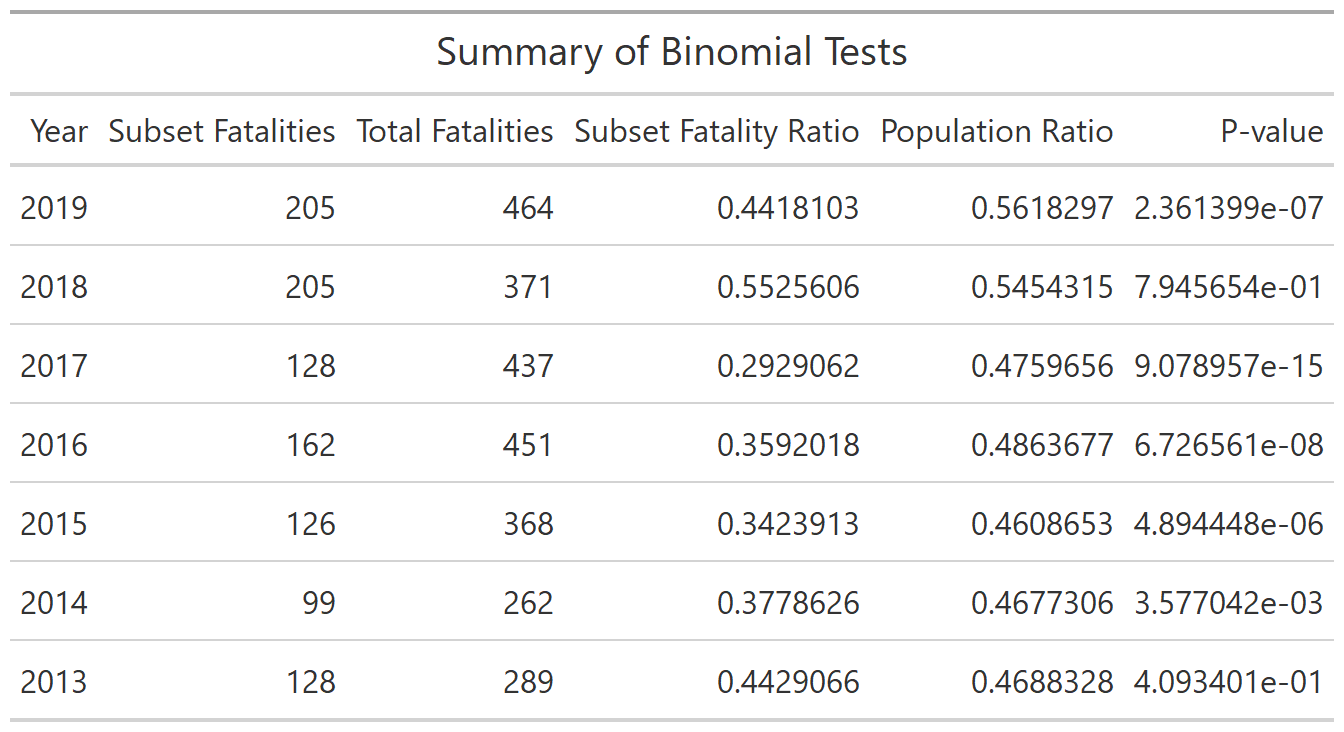
\includegraphics[scale=.4]{Table1.png}\label{Table 1}
 
\subsection{Table 2}
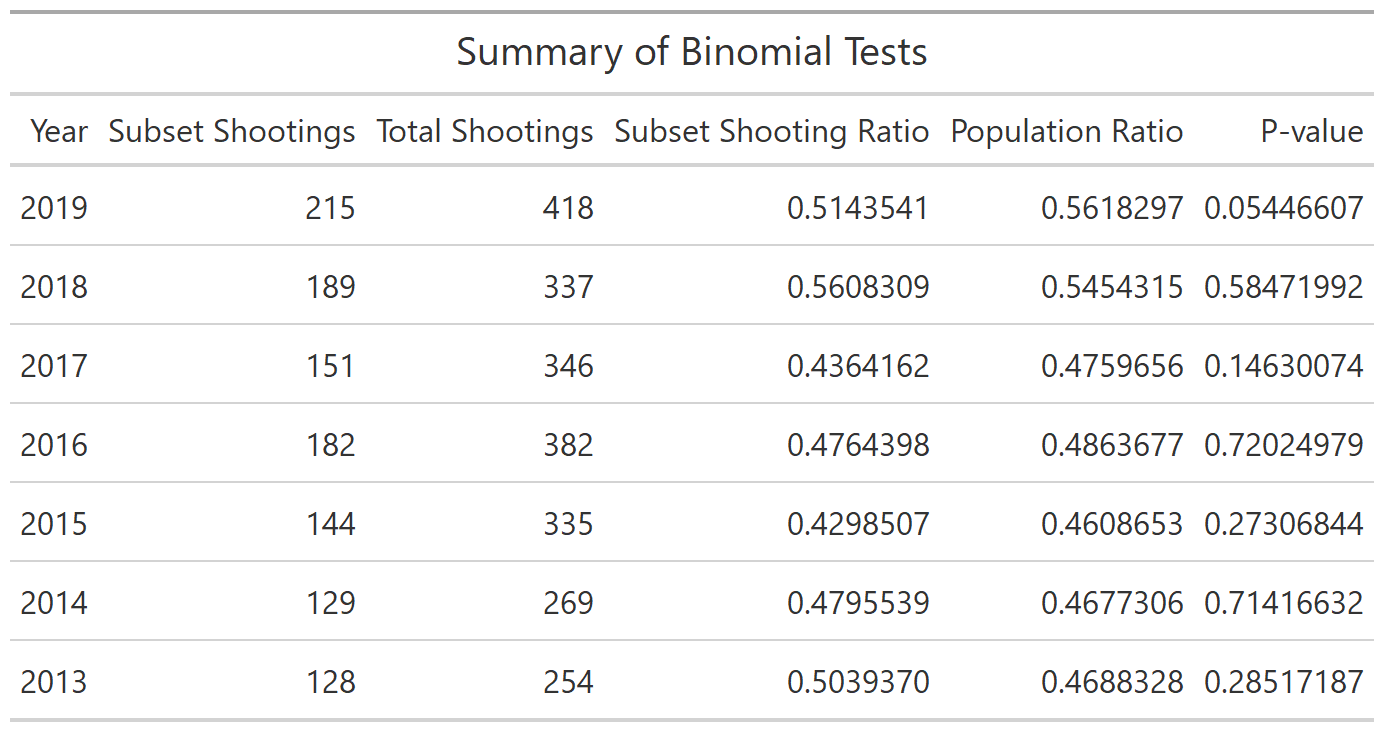
\includegraphics[scale=.4]{Table2.png}\label{Table 2}
 
\subsection{Table 3}
\begin{center}
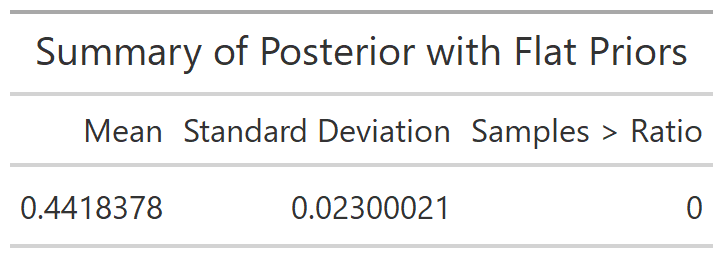
\includegraphics[scale=.5]{Table3.png}\label{Table 3}
\end{center}

\subsection{Table 4}
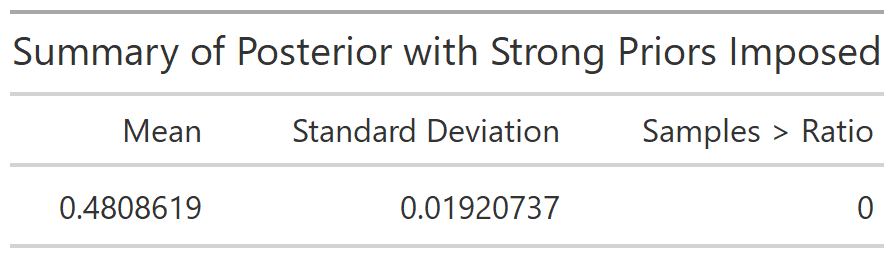
\includegraphics[scale=.5]{Table4.png}\label{Table 4}

\subsection{Table 5}
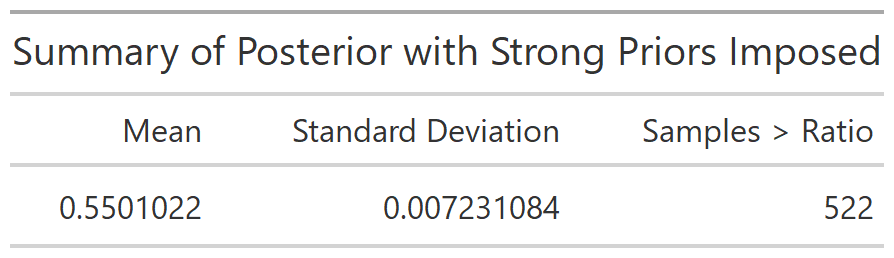
\includegraphics[scale=.5]{Table5.png}\label{Table 5}

\section{Figures}
\subsection{Figure 1}
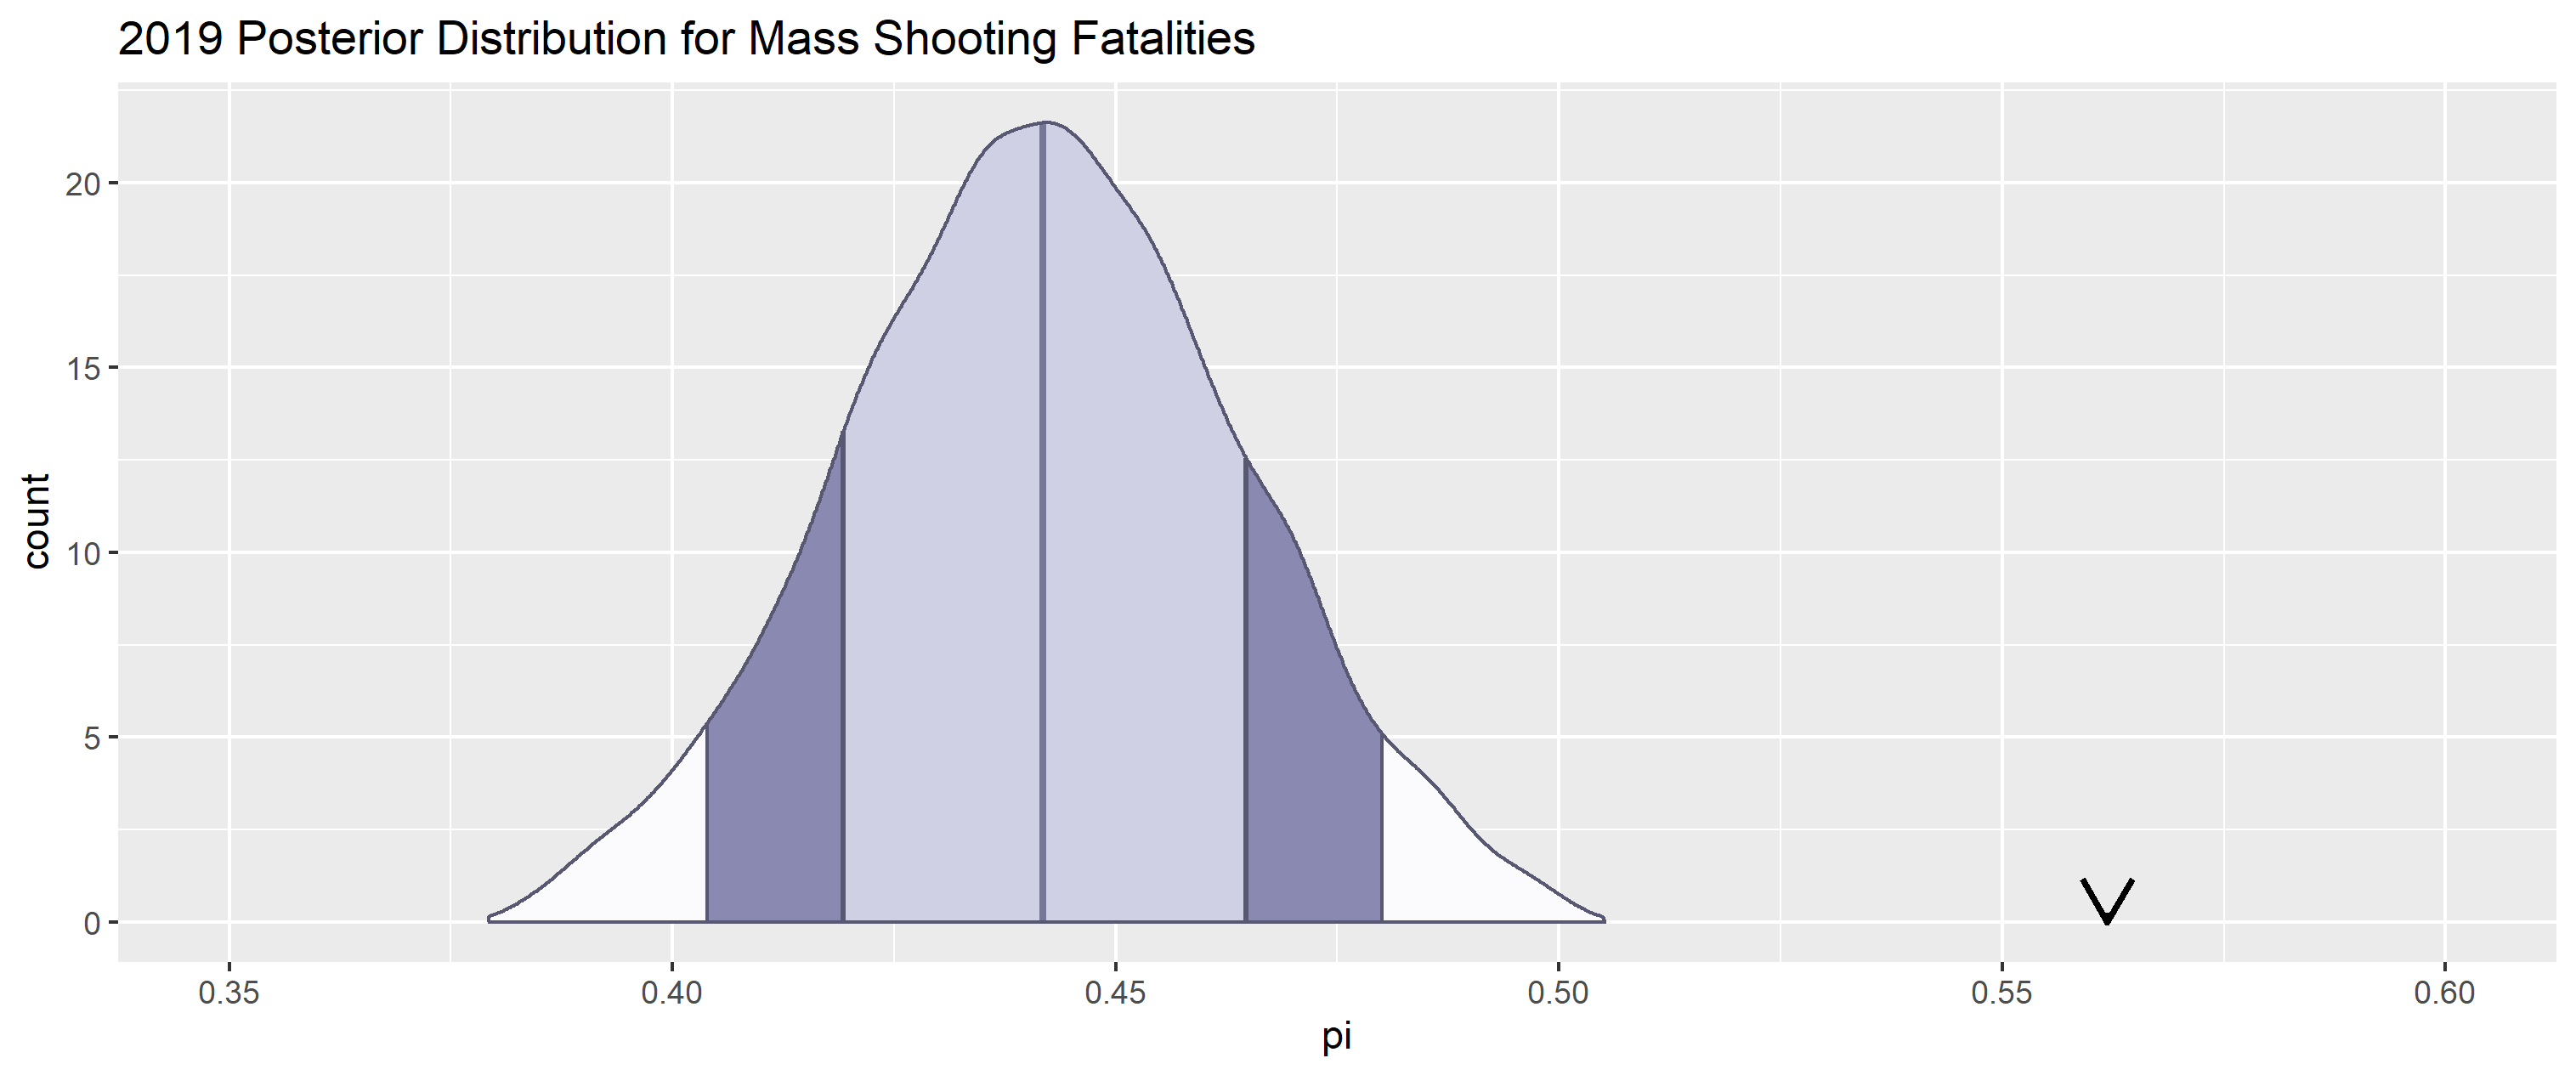
\includegraphics[scale=.5]{Figure1.png}\label{Figure 1}

\subsection{Figure 2}
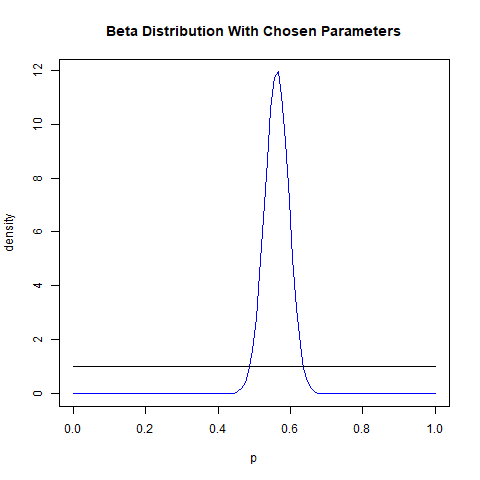
\includegraphics[scale=.6]{Figure2.png}\label{Figure 2}

\subsection{Figure 3}
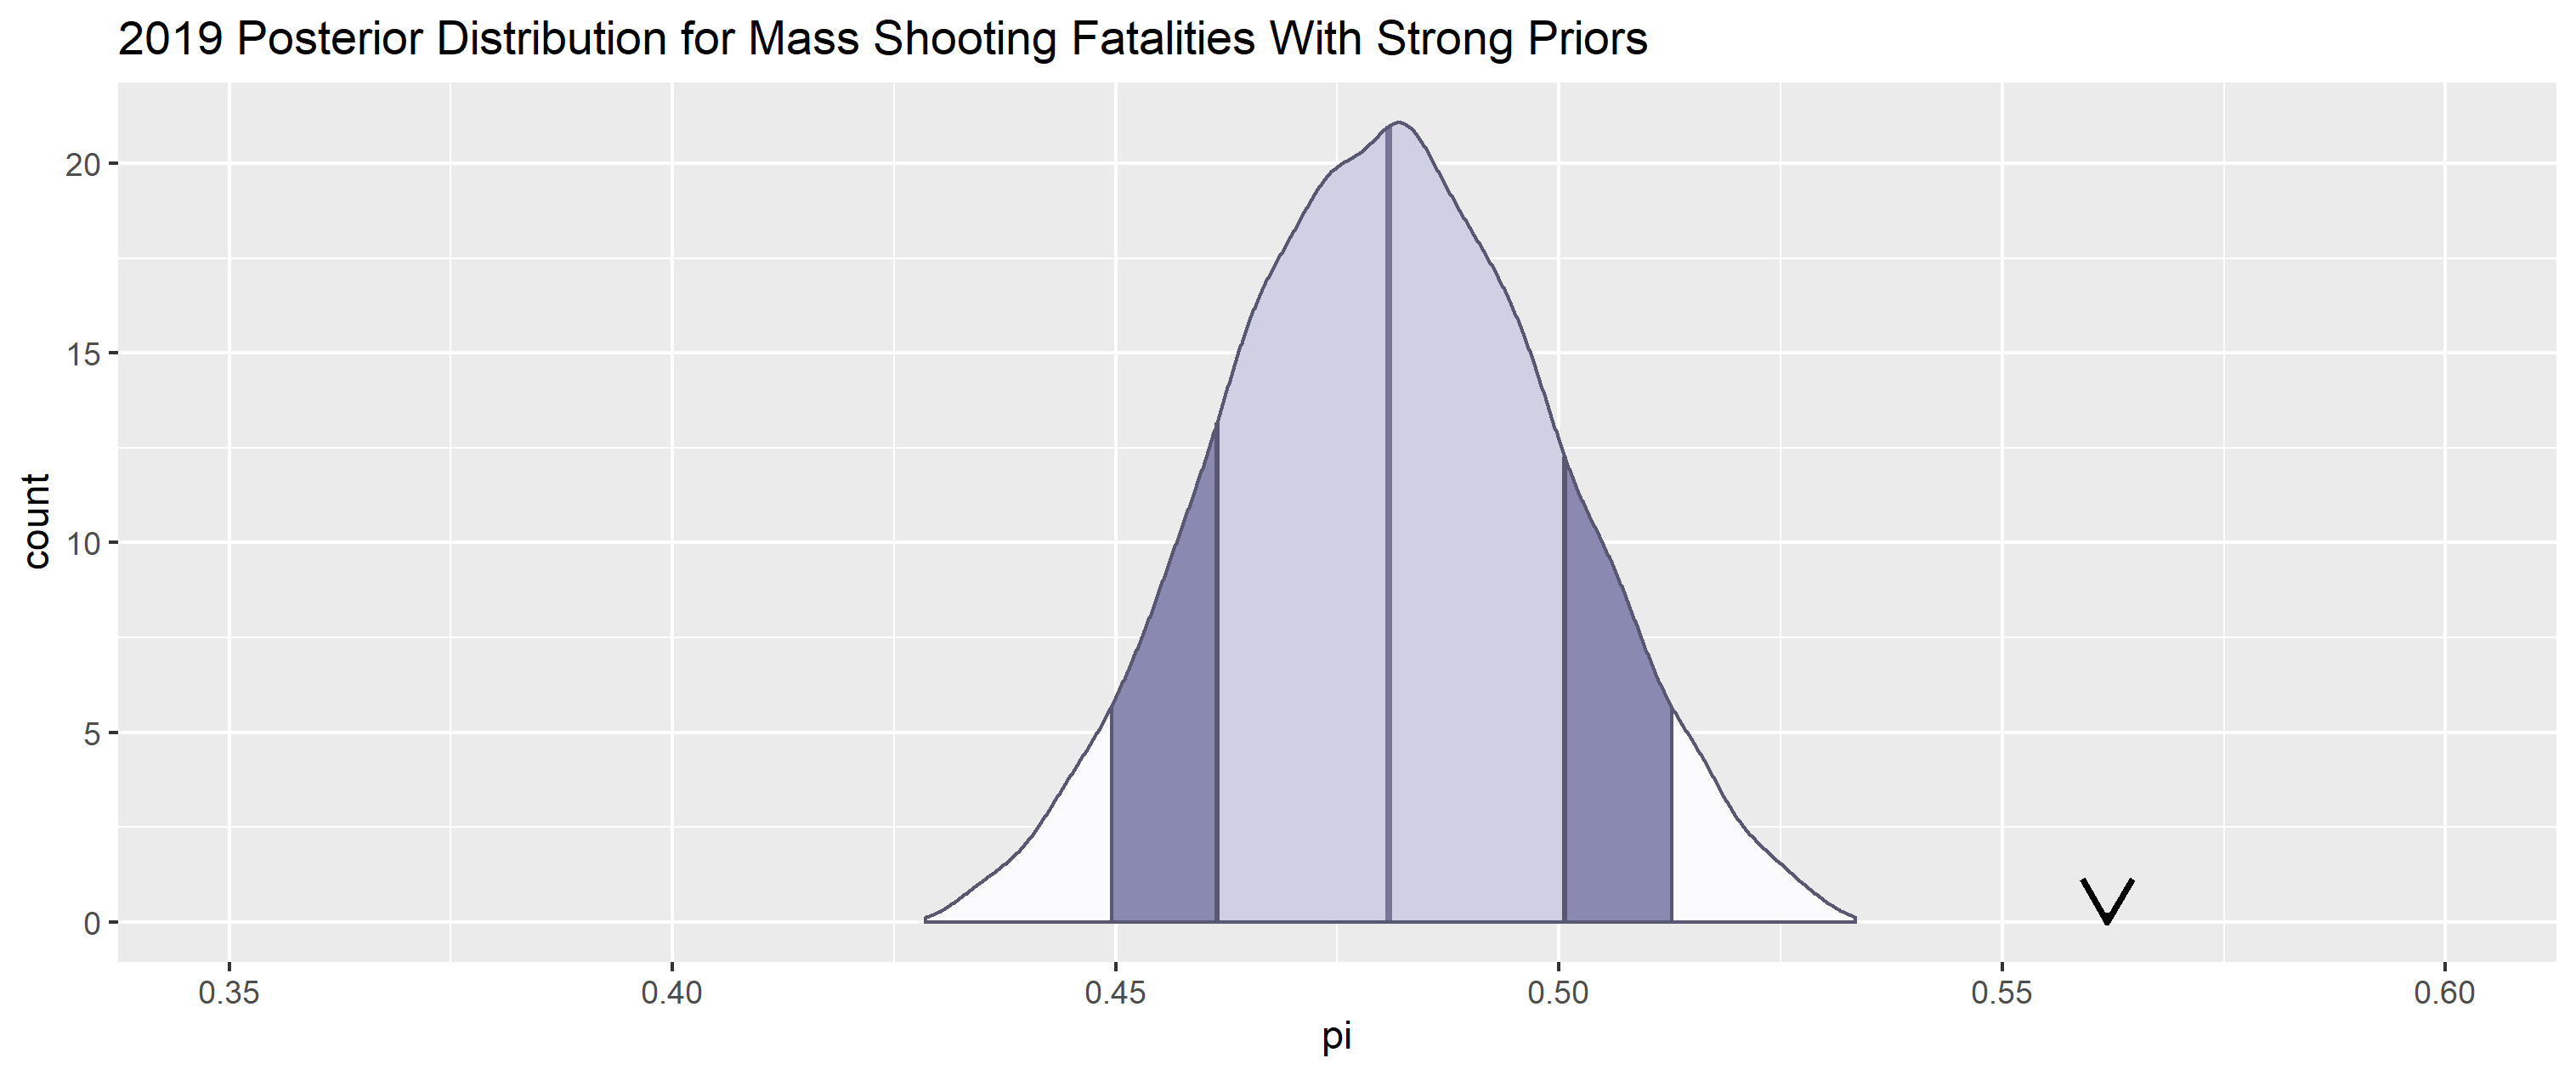
\includegraphics[scale=.5]{Figure3.png}\label{Figure 3}

\subsection{Figure 4}
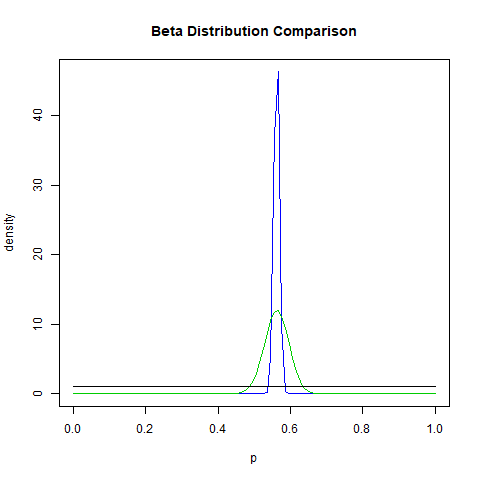
\includegraphics[scale=.75]{Figure4.png}\label{Figure 4}

\subsection{Figure 5}
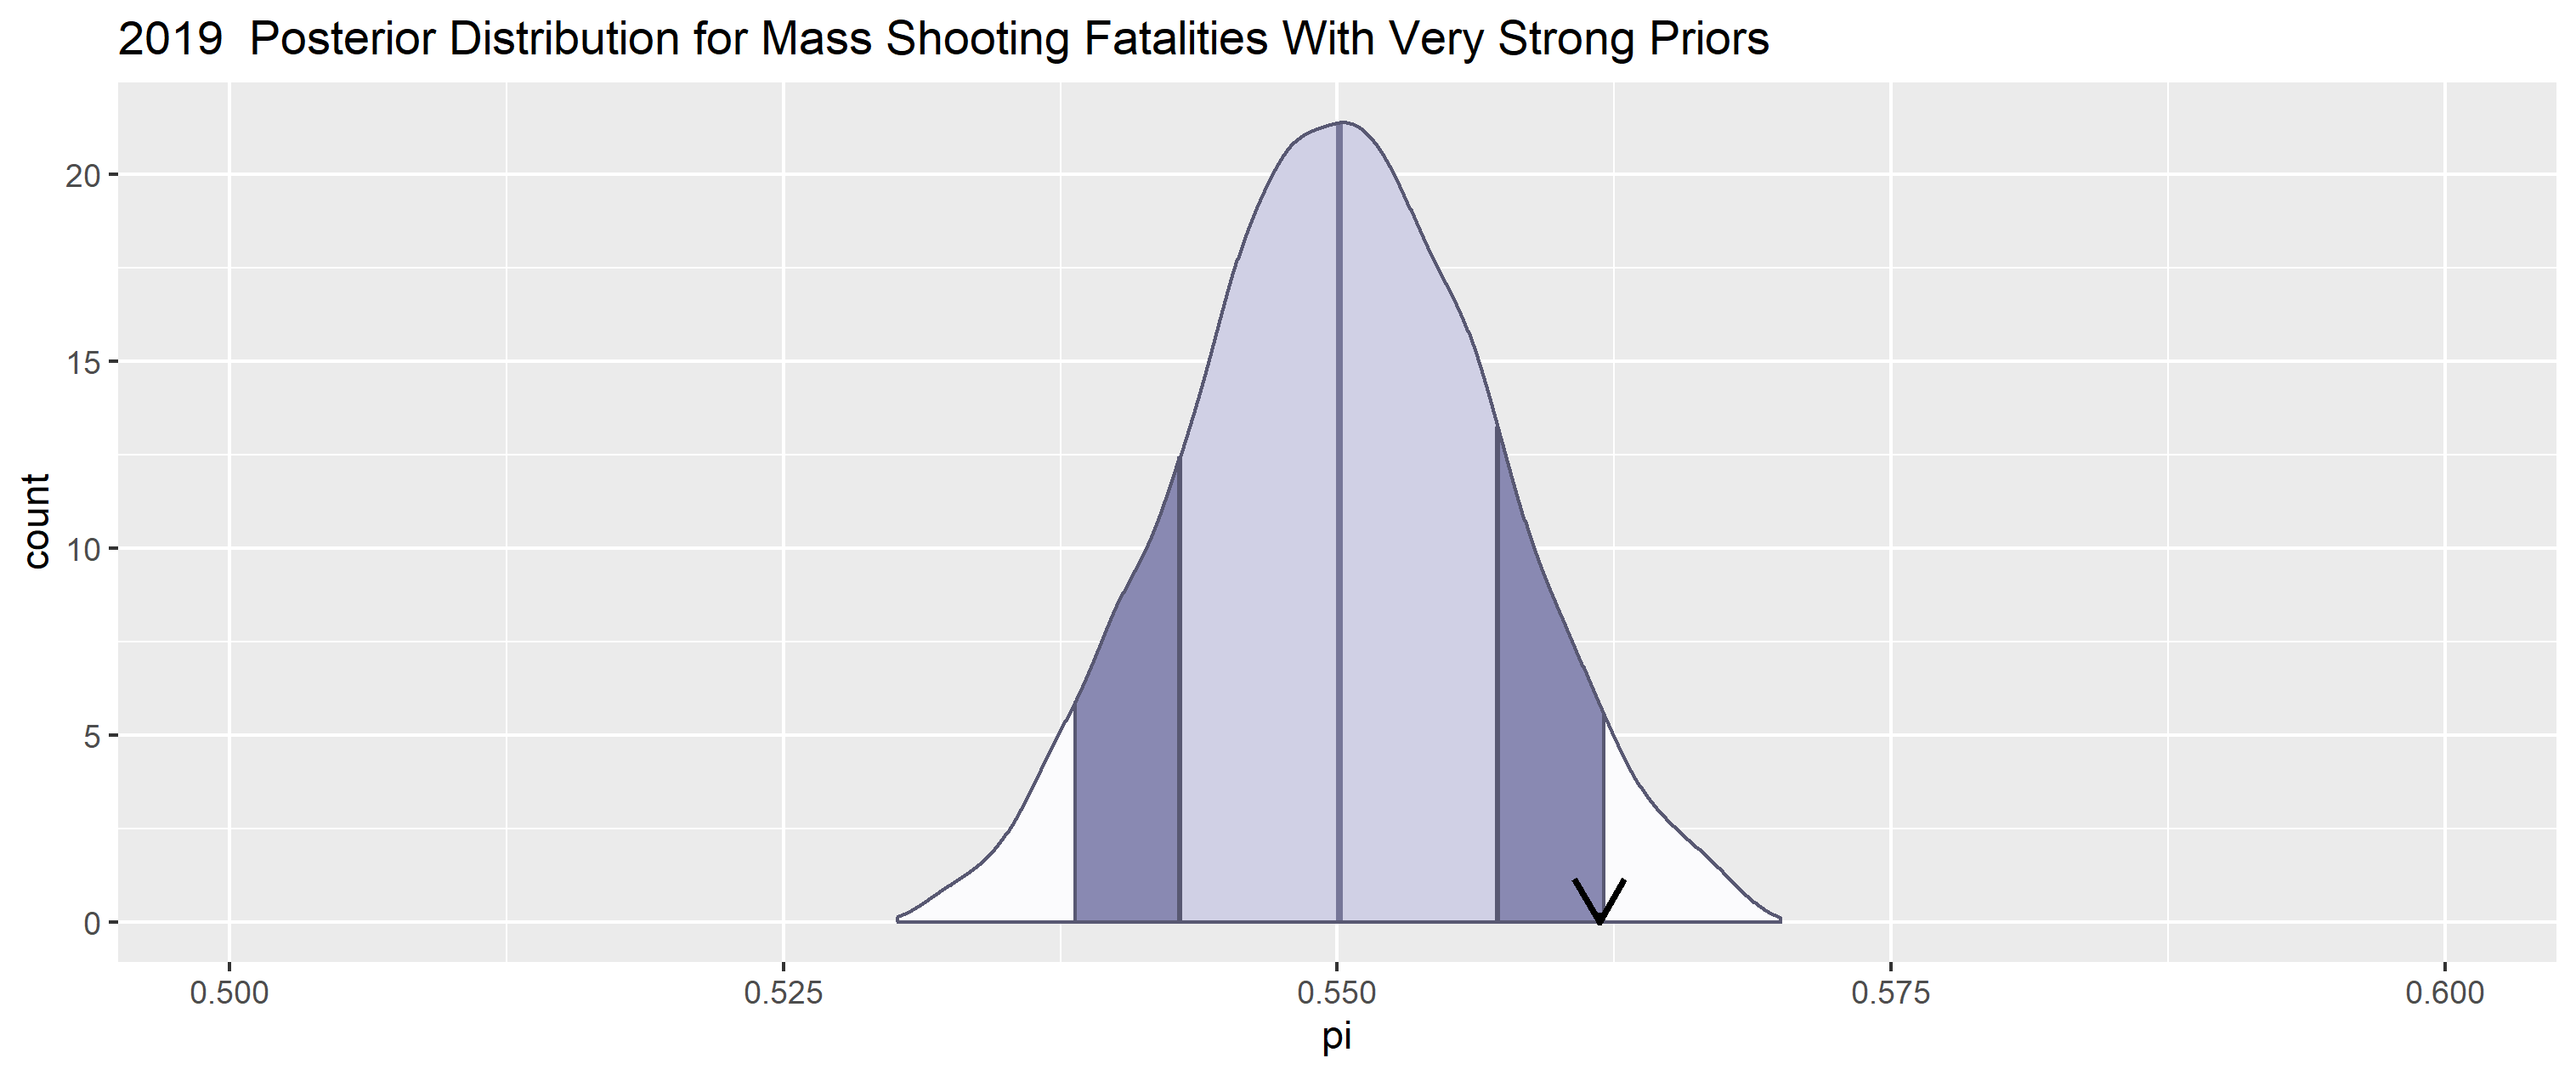
\includegraphics[scale=.5]{Figure5.png}\label{Figure 5}

\section{Appendix B}

\begin{gather*}
\text{Solve the system of equations}\\
Mean(X) = \frac{\alpha}{\alpha + \beta}\\
N = \frac{(\alpha + \beta)^2 (\alpha + \beta +1)}{\alpha \beta}\\
\text{for $\alpha$ and $\beta$ where $N$ and Mean$(X)$ are constants}\\
\text{Let $p = Mean(X)$}\\
p = \frac{\alpha}{\alpha+ \beta}\\
p(\alpha) + p(\beta) = \alpha\\
p(\beta) = (1-p)\alpha\\
\beta = \frac{(1-p)\alpha}{p}\\
\text{Define $\lambda = \frac{1-p}{p}$}
\end{gather*}
\begin{equation}\label{Equation to substitute}
\beta = \lambda \alpha
\end{equation}
\begin{gather*}
\text{We substitute (\ref{Equation to substitute}) into our original system to obtain}\\
N = \frac{((1+\lambda)^2\alpha^2)((1+\lambda)\alpha + 1)}{\lambda \alpha^2}\\
N = \frac{(1+\lambda)^3\alpha^3 + (1+\lambda)^2\alpha^2}{\lambda \alpha^2}\\
N = (1+ \lambda)^2 \alpha + (1+\lambda)^2\\
\frac{N}{(1+\lambda)^2}-1 = \alpha\\
\text{Solving for $\beta$ then becomes trivial.}
\end{gather*}

 

\end{document}


